\chapter{Lecture 13}
\lhead{February 11, 2015}
\chead{21-366 Lambda Calculus Lecture 13}

\section{Normalization}
A question which arises now is how we determine whether two terms are equivalent, for some definition of equivalence. Clearly, for instance, the terms $\l x.X$ and $\l y.X$ share some common structure which the terms $\l xy.X$ and $\l z.Z$ do not. But what do we say about the terms $\l xy.X$ and $X$? Since $\l xy.X \rightarrow_\beta X$, it makes some sort of sense to say that $\l xy.X =_\beta X$ as well. But what about terms with more complicated structure? It is nice, for the purposes of comparison, if we can put terms into some sort of normal form.\\

We say that a term $X$ is \textbf{normal}\index{Normal Term} if it cannot be contracted by $\beta$ reduction. This seems like a natural place to make comparisons from. We have contracted the term as far as we can contract it, and now it cannnot be contracted anymore. Recall that a term is contractable by $\beta$ reduction if it has a $\beta$ redex as a subterm. So we contract all of the $\beta$ redexes to reach normal form. Obviously, this is not possible in all cases; simply consider trying to find a normal form for $\Omega$!\\

$X$ is said to be \textbf{normalizable}\index{Normalizable Term} if there exists a term $N$ in normal form such that $X \twoheadrightarrow_\beta N$. We will eventually prove that this implies some sort of uniqueness about the term $X$. $X$ is said to be \textbf{strong normalizable}\index{Strong Normalizable Term} if every reduction sequence of $X$ ultimately ends in a normal form term. We indicate that $X$ is strongly normalizable by $X \in \hbox{SN}$.\\

To understand why the distinction between normalizable and strong normalizable is necessary, consider the term $Kx\Omega$. There are two possible $\beta$ reductions:
\begin{eqnarray*}
  Kx\Omega &\rightarrow_\beta& x\\
  Kx\Omega &\rightarrow_\beta& Kx(\Omega\Omega)
\end{eqnarray*}
Clearly, one of these reduction sequences terminates in the normal term $x$. The term $Kx(\Omega\Omega)$, however, is in the same situation as $Kx\Omega$. By reducing the $K$ first, we can return to our normal form $x$. However areduction sequence which consists of the repeated reduction of $\Omega$ will never terminate in a normal form. It is worth noting as well that if a reduction sequence of $Kx\Omega$ ever does terminate, it terminates in the form $x$. You might recall that this is simply our weak diamond property.
\begin{center}
  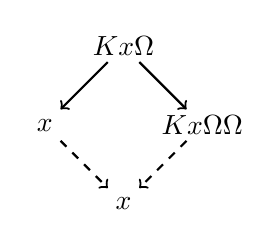
\begin{tikzpicture}
    \draw (0,0) node {$Kx\Omega$};
    \draw (-1,-1) node {$x$};
    \draw (1,-1) node {$Kx\Omega\Omega$};
    \draw (0,-2) node {$x$};
    \draw[thick, ->] (-.2,-.2) -- (-.8,-.8);
    \draw[thick, ->, dashed] (-.8,-1.2) -- (-.2,-1.8);
    \draw[thick, ->] (.2,-.2) -- (.8,-.8);
    \draw[thick, ->, dashed] (.8,-1.2) -- (0.2,-1.8);
  \end{tikzpicture}
\end{center}

\subsection{Reduction Sequences of Strongly Normalizable Terms}
We claim that if $X$ is strongly normalizable, then the entire reduction tree of $X$ is finite, and the tree ends in a unique normal form $W$.
\begin{center}
  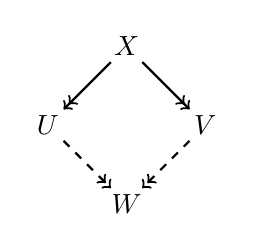
\begin{tikzpicture}
    \draw (0,0) node {$X$};
    \draw (-1,-1) node {$U$};
    \draw (1,-1) node {$V$};
    \draw (0,-2) node {$W$};
    \draw[thick, ->>] (-.2,-.2) -- (-.8,-.8);
    \draw[thick, ->>, dashed] (-.8,-1.2) -- (-.2,-1.8);
    \draw[thick, ->>] (.2,-.2) -- (.8,-.8);
    \draw[thick, ->>, dashed] (.8,-1.2) -- (0.2,-1.8);
  \end{tikzpicture}
\end{center}

We can prove the first claim by appealing to K\"onig's lemma. A finitely long term can only have a finite number of possible reductions. Since the term is strongly normalizable, we know that by definition every reduction sequence terminates in a normal form. That they terminate implies that there are no infinite paths.\\

Our second claim is more sophisticated. We can prove it by induction on the length of the reduction sequences of $X$. The trivial case is when $X$ is already normal, and the length of all $\beta$ reduction sequences of $X$ are $0$. In our inductive step, consider reduction sequences $R_1$ and $R_2$ from $X$ to $U$ and $V$:
\begin{eqnarray*}
  R_1: X \twoheadrightarrow_\beta U\\
  R_2: X \twoheadrightarrow_\beta V\\
\end{eqnarray*}

If the lengths of $R_1$ or $R_2$ are not one (or zero), then we can look at the first reductions of $R_1$ and $R_2$. If one of $R_1$ or $R_2$ are zero, then one reduction could be the pseudo-$\beta$ reduction of a term to itself.

\begin{center}
  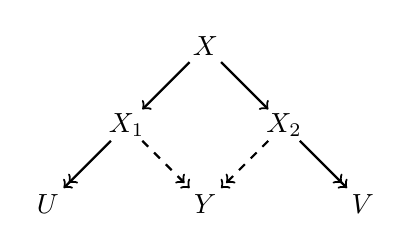
\begin{tikzpicture}
    \draw ( 0, 0) node {$X$};
    \draw (-1,-1) node {$X_1$};
    \draw ( 1,-1) node {$X_2$};
    \draw ( 0,-2) node {$Y$};
    \draw (-2,-2) node {$U$};
    \draw ( 2,-2) node {$V$};

    \draw[thick, ->] (-0.2,-0.2) -- (-0.8,-0.8);
    \draw[thick, ->>, dashed] (-0.8,-1.2) -- (-0.2,-1.8);
    \draw[thick, ->] (0.2,-0.2) -- (0.8,-0.8);
    \draw[thick, ->>, dashed] (0.8,-1.2) -- (0.2,-1.8);
    \draw[thick, ->>] (-1.2,-1.2) -- (-1.8,-1.8);
    \draw[thick, ->>] (1.2,-1.2) -- (1.8,-1.8);
  \end{tikzpicture}
\end{center}

Observe that $X_1$ has a smaller reduction tree than $X$. We can then use the induction hypothesis to see that $U$ and $Y$, and $V$ and $Y$ reduce to some terms $U_1$ and $V_1$:

\begin{center}
  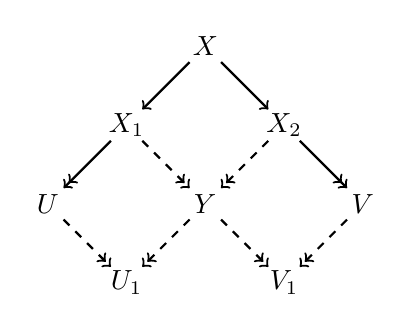
\begin{tikzpicture}
    \draw ( 0, 0) node {$X$};
    \draw (-1,-1) node {$X_1$};
    \draw ( 1,-1) node {$X_2$};
    \draw ( 0,-2) node {$Y$};
    \draw (-2,-2) node {$U$};
    \draw ( 2,-2) node {$V$};
    \draw (-1,-3) node {$U_1$};
    \draw ( 1,-3) node {$V_1$};

    \draw[thick, ->] (-0.2,-0.2) -- (-0.8,-0.8);
    \draw[thick, ->>, dashed] (-0.8,-1.2) -- (-0.2,-1.8);
    \draw[thick, ->] (0.2,-0.2) -- (0.8,-0.8);
    \draw[thick, ->>, dashed] (0.8,-1.2) -- (0.2,-1.8);
    \draw[thick, ->>] (-1.2,-1.2) -- (-1.8,-1.8);
    \draw[thick, ->>] (1.2,-1.2) -- (1.8,-1.8);

    \draw[thick,->>,dashed] (-1.8,-2.2) -- (-1.2,-2.8);
    \draw[thick,->>,dashed] ( 1.8,-2.2) -- ( 1.2,-2.8);
    \draw[thick,->>,dashed] ( 0.2,-2.2) -- ( 0.8,-2.8);
    \draw[thick,->>,dashed] (-0.2,-2.2) -- (-0.8,-2.8);
  \end{tikzpicture}
\end{center}

We now have $U_1$ and $V_1$, which by the inductive hypothesis eventually reduce to some term $W$ in a finite number of reductions. Additionally, that number of reductions is fewer than the number of reductions for $X$, so by the induction hypothesis we can claim that there exist reductions $U_1 \twoheadrightarrow_\beta W$ and $V_1 \twoheadrightarrow_\beta W$.

\begin{center}
  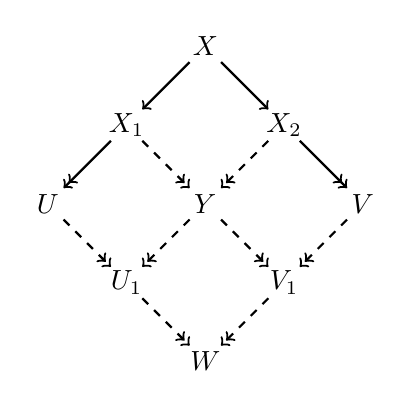
\begin{tikzpicture}
    \draw ( 0, 0) node {$X$};
    \draw (-1,-1) node {$X_1$};
    \draw ( 1,-1) node {$X_2$};
    \draw ( 0,-2) node {$Y$};
    \draw (-2,-2) node {$U$};
    \draw ( 2,-2) node {$V$};
    \draw (-1,-3) node {$U_1$};
    \draw ( 1,-3) node {$V_1$};
    \draw ( 0,-4) node {$W$};

    \draw[thick, ->] (-0.2,-0.2) -- (-0.8,-0.8);
    \draw[thick, ->>, dashed] (-0.8,-1.2) -- (-0.2,-1.8);
    \draw[thick, ->] (0.2,-0.2) -- (0.8,-0.8);
    \draw[thick, ->>, dashed] (0.8,-1.2) -- (0.2,-1.8);
    \draw[thick, ->>] (-1.2,-1.2) -- (-1.8,-1.8);
    \draw[thick, ->>] (1.2,-1.2) -- (1.8,-1.8);

    \draw[thick,->>,dashed] (-1.8,-2.2) -- (-1.2,-2.8);
    \draw[thick,->>,dashed] ( 1.8,-2.2) -- ( 1.2,-2.8);
    \draw[thick,->>,dashed] ( 0.2,-2.2) -- ( 0.8,-2.8);
    \draw[thick,->>,dashed] (-0.2,-2.2) -- (-0.8,-2.8);
    
    \draw[thick,->>,dashed] (-0.8,-3.2) -- (-0.2,-3.8);
    \draw[thick,->>,dashed] ( 0.8,-3.2) -- ( 0.2,-3.8);
  \end{tikzpicture}
\end{center}

This demonstrates that all reduction sequences of $X$ eventually terminate at some term $W$, which proves our claim. So all redution sequences of strongly normalizable terms are finite, and terminate in the same term.

\section{Simulating Strong Normalization}

\textbf{Digression:} $\infty$ reduction paths (or perpetual reduction paths). For some $X \not\in$ SN, find a principle redex in $X$, called $\Delta$ such that the contraction of $\Delta$ results in a term $Y \not\in$ SN.\\

Possible terms:
\begin{enumerate}
  \item The principle redex of $\l uU$ is the principle redex of $U$.
  \item $X = X_1,\ldots X_n$ has a principle redex of $X_i$ such that $i$ is the smallest such $i$ such that a redex exists.
  \item $X = (\l xX_0)X_1,\ldots,X_n$. If the head redex is contracted, then it is principle.
\end{enumerate}
The principle redex redex is

\begin{enumerate}[a.]
  \item if $x \not\in FV(X_0)$, then the principle redex of $X$ is the principle redex of $X_1$, if it exists.
  \item else $(\l xX_0)X_1$ is the principle redex.
\end{enumerate}

\textbf{Corollary:} If $X$ is not strongly normalizable, and $Y$ results by contracting the principle redex of $X$, then $Y \not\in$ SN.\\

\textbf{Definition:} Comparing redexes in $X$. Standardizations says that you should always contract a redex able on to the left of the anchor.

\subsection{On Coloring Redexes (A Simulation of SN)}
Given a term $X$, we color some (strict) subset of the redexes in $X$ green. An uncolored redex is red. If $X$ reduces to $Y$ in a single step by some green redex $\Delta$, then the redexes in $Y$ which are residuals of those in $X$ which are green get colored green. We call this a \textbf{Colored Reduction}\index{Colored Reduction|textbf}.\\

If $X \rightarrow_{\beta, colored} Y$, and $Y$ has no colored redexes, then $Y$ is said to be a complete development of green redexes in $X$.\\

\textbf{Theorem (Hindley):}\index{Hindley's Theorem} Every colored reduction sequence terminates in a unique normal form. Note that we have weak diamond for colored reductions.
\begin{center}
  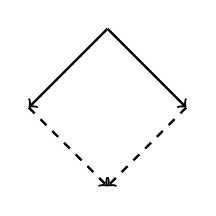
\begin{tikzpicture}
    \draw[thick, ->] (0,0) -- (-1,-1); % X
    \draw[thick, ->, dashed] (-1,-1) -- (0,-2); % U by Delta_1
    \draw[thick, ->] (0,0) -- (1,-1); % V by Delta_2
    \draw[thick, ->, dashed] (1,-1) -- (0,-2); % W by residuals of Delta_1 and Delta_2
  \end{tikzpicture}
\end{center}

\textbf{Proof:} $X \mapsto \# X$ and a colored reduction to $Y$ gives us $Y \mapsto \# Y$ for some $\#$ which associates a nonnegative integer with terms.